\chapter{Prüfstand}
\section{Grundlagen des Prüfstandes}
In diesem Kapitel wird der verwendete Schaltaktorikprüfstand des IMS vorgestellt, an dem  die Entwicklung des Smart Actuators stattgefunden hat. Die Konstruktion des Prüfstandes erfolgte in vorangegangenen Arbeiten und wurde seitdem stetig weiterentwickelt. An ihm werden Schaltaktoriksysteme für Fahrzeugantriebe untersucht. Abbildung \ref{fig:Pruefstand} zeigt die in dieser Arbeit verwendeten Subsysteme des Prüfstandes. Im Folgenden erfolgt zunächst die Vorstellung des mechanischen Aufbaus, woraufhin der elektronische Aufbau anschließt. 

\begin{figure}[h]
	\centering
<<<<<<< HEAD
		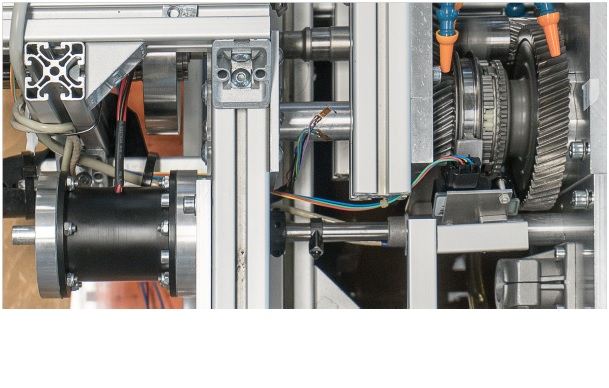
\includegraphics{Bilder/Pruefstand.jpg}
=======
	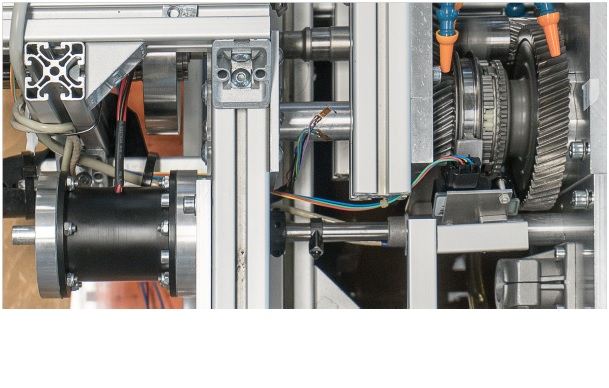
\includegraphics{./Bilder/Pruefstand.jpg}
>>>>>>> cc7043c638d4a861f6d73a6ccf59b0ffca8d4bdd
	\caption{Prüfstand}
	\label{fig:Pruefstand}
\end{figure}

\subsection{Getriebe allgemein}

Ein Getriebe ist im Automobil dafür zuständig, die Drehzahl des Motors in ein Drehmoment umzuwandeln, welches die Räder antreibt. Da Motoren nur einen kleinen Bereich von Motordrehzahlen abdecken werden mehrstufige Getriebe verwendet, die verschiedene Raddrehzahlen durch unterschiedliche Übersetzungsverhältnisse bereitstellen können.  Das Einstellen des jeweiligen Ganges kann dabei per Hand (Handschaltgetriebe) oder automatisiert über einen Aktor (Schaltaktorik) erfolgen. 
Im Fahrzeuggetriebe, beispielhaft dargestellt in \ref{fig:Fahrzeuggetriebe} ist die Eingangswelle, welche durch den Motor angetrieben wird, über eine Zahnradverbindung  fest mit der  Vorgelegewelle verbunden. Auf ihr sind noch weitere fest fixierte Zahnräder angebracht, deren Anzahl mit den verfügbaren Gängen übereinstimmt. Diese greifen jeweils in Losräder auf der Abtriebswelle. Um einen bestimmten Gang einzulegen muss nun das jeweilige Losrad für den Moment fest mit der Abtriebswelle verbunden werden, sodass nur diese Zahnverbindung ein Drehmoment überträgt. Dies geschieht über eine formschlüssige Verbindung mit einer Schaltmuffe, die über die durch den Aktor angetrieben Schaltgabel in Position gebracht wird.

\begin{figure}[h]
	\centering
		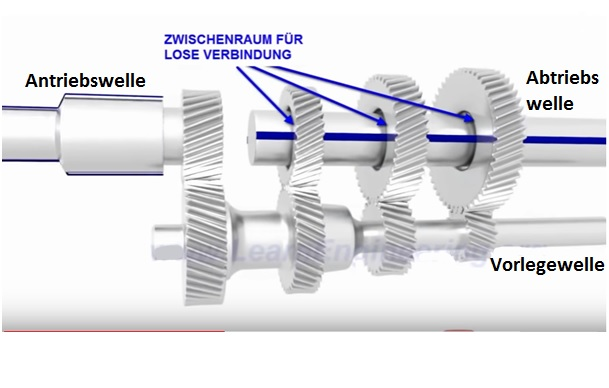
\includegraphics{Bilder/Fahrzeuggetriebe.jpg}
	\caption{Fahrzeuggetriebe}
	\label{fig:Fahrzeuggetriebe}
\end{figure}

\subsection{Getriebe des Prüfstands}

Der Prüfstand besitzt zwei Gänge, in die über eine Schaltgabel geschaltet werden kann. Eine Bewegung der Schaltgabel nach links legt Gang 1 über eine mechanische Synchronisierung ein, während mit Hilfe einer Bewegung nach rechts die Schaltung des Ganges 2 durch eine Klauenkupplung erfolgt. Somit können sowohl Schaltaktoriksysteme mit als auch ohne Synchronring untersucht werden.
Die Bewegung der Schaltgabel wird durch einen Linearaktor ermöglicht, welcher von außen an das Item-Profil verschraubt ist. In diesem ist eine Tauchspule verbaut, die die benötigten Kräfte auf die Läuferstange aufbringt. Über eine starre Wellenkupplung sind Läuferstange und Schaltgabel miteinander verbunden, wodurch die Kräfte auf die Schaltgabel übertragen werden und Schaltvorgänge ermöglicht werden.

\subsection{Aktor}

Der in dem Prüfstand verbaute Tauchspulenaktor wurde von Oliver Hahn im Rahmen seiner Bachelorthesis entwickelt und konstruiert. Er übernimmt die Aufgabe, die Schaltgabel  über die Schaltstange translatorisch zu verschieben. Sein Querschnitt ist in folgender Abbildung schematisch dargestellt.

\begin{figure}[h]
	\centering
		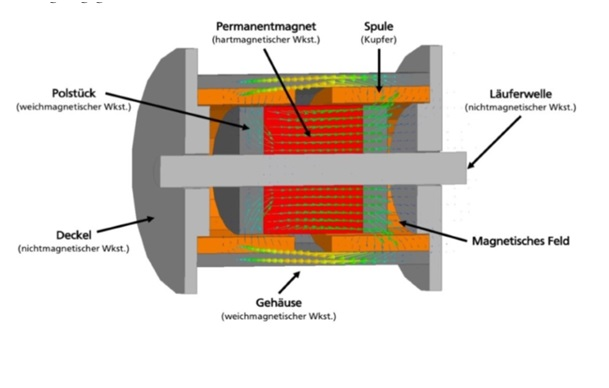
\includegraphics{Bilder/Querschnitt Aktor.jpg}
	\caption{Querschnitt Tauchspulenaktor}
	\label{fig:Querschnitt Aktor}
\end{figure}

Sein Aufbau ist zylindrisch und kann in den ortsfesten Stator und den beweglichen Läufer unterteilt werden. Der Stator des Aktors besteht aus zwei in Reihe geschalteten Kupferspulen, welche fest in dem Gehäuse aus Weicheisen liegen und nach oben und unten mit Deckeln aus Aluminium fixiert werden. Der Läufer besteht aus einer nichtmagnetischen Läuferwelle, auf der sich fünf Permanentmagneten aus Neodym-Eisen-Bor befinden, welche mit Hilfe von zwei Polstücken aus Weicheisen axial auf der Läuferstange montiert sind. 
Werden nun die Kupferspulen von Strom durchflossen, so wirkt eine vom Magnetfeld der Permanentmagneten induzierte Lorentzkraft orthogonal auf sie. Diese Kraft ist abhängig von der Stromstärke I, der magnetischen Flussdichte der Permanentmagneten B und der vom Magnetfeld durchsetzten Leiterlänge l:
	\[F=I*l*B
\]


